% !TeX encoding = UTF-8
% !TeX spellcheck = en_GB
% !TeX root = ../thesis.tex

\chapter{Methodology}\label{ch:methodology}
This chapter introduces the research methodology and review protocol that is based on the systematic literature review (SLR) (in Section~\ref{sec:slr}) and used in order to search for the needed primary studies to answer the following research questions in Section~\ref{sec:research_questions}. The taxonomy that is needed to gather information from the collection of studies is then defined in Section~\ref{sec:taxonomy}.


\section{Systematic Literature Review}\label{sec:slr}
According to Kitchenham et al.~\cite{Kitchenham2007} SLR is an analysis of publications about a certain topic that collects and critically evaluates multiple research studies or papers in a systematic way. Its purpose is to provide an exhaustive summary of the available literature relevant to a specific research question in a transparent and reproducible way. The following points utilize the review protocol that is used to conduct the literature review in a strategic manner and consist of the research questions that should be answered, selection criteria the found papers need to fulfil and a search strategy on how to browse databases in order to find the most relevant publications.

\subsection{Research Questions}\label{sec:research_questions}
This thesis aims to answer the following research questions (RQs):

\begin{enumerate}
	\item[RQ1] Which layer in the IoT World Forum Reference Model is covered by the least security patterns?
	\item[RQ2] Which security goal is addressed by security patterns the least and how can the coverage be improved?
	\item[RQ3] How many of the OWASP top ten most common IoT vulnerabilities are solved by utilizing these security patterns?
\end{enumerate}

\subsection{Selection Criteria}
To minimize bias in the search and selection of our primary studies for this master's thesis, we predefined guidelines that need to be fulfilled for a study to be used in our analysis. This approach leads us to the following inclusion and exclusion criteria:

\subsubsection{Inclusion Criteria:}\label{subsubsec:ICs}
\begin{enumerate}
	\item[IC1] A primary study must contain (one or more) security pattern that is applicable to an IoT system.
	\item[IC2] A primary study must target the IoT field, either in a general or specific application domain of IoT.
	\item[IC3] A primary study must discuss security objectives for system design, architecture or infrastructure.
\end{enumerate}

\subsubsection{Exclusion Criteria:}\label{subsubsec:ECs}
\begin{enumerate}
	\item[EC1] Papers not written in the English language are filtered out.
	\item[EC2] Papers that discuss design, privacy or misuse patterns as well as security architectures for the IoT domain are excluded.
	\item[EC3] Papers that are not peer-reviewed are also ruled out. 
\end{enumerate}
 

\subsection{Search and Selection Strategy}
This section focuses on the selection of appropriate primary studies that can serve as a basis to answer the aforementioned research questions. The goal is to collect as many primary studies as possible that are relevant for this thesis. The strategy to find papers that discuss security patterns is divided into two main parts: automatic and manual search. First we let a set of search engines find example studies in an automated approach with specific keywords. Here we also apply the mentioned inclusion and exclusion criteria to exclude any unwanted results ahead of time. Second we conduct a manual search in order to fill the gaps with any relevant scientific papers that were missed by the machine. In an attempt to avoid duplicates, the last stage of the search process consists of merging identical papers that were found by different search engines. The exact procedure is described in the following points and illustrated in Figure~\ref{fig:search-overview}.

\subsubsection{1. Database search:} 
As our primary search engines, we utilized five well known databases for scientific publications: IEEE Xplore\footnote{\href{https://ieeexplore.ieee.org}{https://ieeexplore.ieee.org, last accessed: 21.05.2022.}}, ACM Digital Library\footnote{\href{https://dl.acm.org}{https://dl.acm.org, last accessed: 21.05.2022.}}, ScienceDirect\footnote{\href{https://www.sciencedirect.com}{https://www.sciencedirect.com, last accessed: 21.05.2022.}}, Web of Science\footnote{\href{https://access.clarivate.com}{https://access.clarivate.com, last accessed: 21.05.2022.}} and Scopus\footnote{\href{https://www.scopus.com}{https://www.scopus.com, last accessed: 21.05.2022.}}. Because Scopus and ACM Digital Library already reference SpringerLink\footnote{\href{https://link.springer.com}{https://link.springer.com, last accessed: 21.05.2022.}}, we could exclude the former as well as Researchgate\footnote{\href{https://www.researchgate.net}{https://www.researchgate.net, last accessed: 21.05.2022.}} and Google Scholar\footnote{\href{https://scholar.google.com}{https://scholar.google.com, last accessed: 21.05.2022.}} which also include many non-peer-reviewed and non-English papers. Based on Kitchenham et al.~\cite{Kitchenham2007} we created keywords that generate papers that are relevant for the answers to our research questions. This led us to the following search query that was used for our initial database search on May 21st, 2022: 
\begin{center}
	(\emph{\q{Internet of Things}} \textbf{OR} \emph{\q{IoT}} \textbf{OR}  \emph{\q{Cyber Physical Systems}} \textbf{OR} \emph{\q{Web of Things}}) \\ \textbf{AND} \\
	(\emph{\q{Security Pattern}} \textbf{OR} \emph{\q{Security Design Pattern}})	
\end{center}	
For each search the query string needed to be slightly modified to fit each database's advanced search functionality and guidelines.
	
\subsubsection{2. Manual search:} 
By utilizing the snowballing strategy that was introduced by Wholin and Prikladnicki~\cite{Wohlin2013}, we searched manually for further literature that was missed by the automatic database inquiry. Following references of the already found papers, we looked for relevant publications that include further security design patterns that can be useful for our study. After a few iterations we found a set of papers that met the inclusion criteria of our SLR. After eliminating any duplicates of papers that were already discovered by the initial database search, we could add eleven more articles to our database search result. By including these manual publication findings, our RQs can be answered in a more thorough way. 

\begin{figure}[ht]
	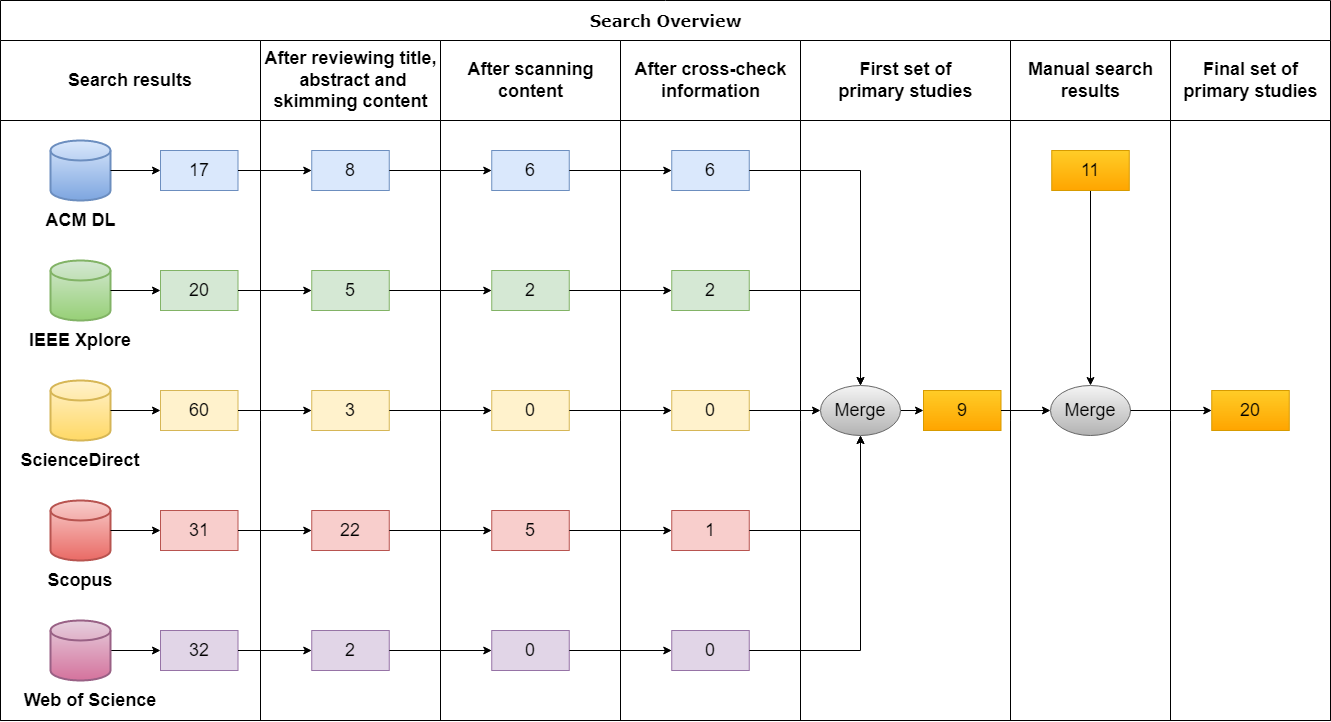
\includegraphics[scale=0.3]{img/search}
	\centering
	\caption{Overview of the search and selection procedure}
	\label{fig:search-overview}
\end{figure}


\section{Taxonomy of the Research Area}\label{sec:taxonomy}
In this section the taxonomy of IoT security patterns is introduced. The main purpose of the taxonomy classifications is to simplify the extraction and comparison of patterns that are described in the primary studies. Subsection~\ref{subsec:posa} defines a scheme on how to structure the pattern descriptions, then Subsection~\ref{subsec:model} depicts what the general architecture of an IoT system looks like and Subsection~\ref{subsec:security} shows which security goals are the main focus of the extracted patterns as the last part of the taxonomy classifications.

\subsection{Pattern Description with POSA}\label{subsec:posa}
All patterns in the catalogue will be listed utilizing the Pattern-Oriented Software Architecture (POSA) form, so that the descriptions of IoT security patterns in this master's thesis are presented in a unified form. Although POSA is a popular format, not all patterns in the analysed publications are presented in this way or do have a standardized format at all. Another very popular form is Gang of Four (GoF) which is used in the \q{Design Patterns: Elements of Reusable Object-Oriented Software} book~\cite{Gamma1994}. But we chose POSA because it is a well-accepted and widely used pattern description format that provides standard templates~\cite{Bunke2014} and is used in the book with the same name by Buschmann et al.~\cite{Buschmann1996}. Other pattern description formats can also be easily converted and mapped to the POSA form that describes design patterns with the following keywords: \emph{Intent, Example, Context, Problem, Structure, Solution, Dynamics, Consequences, Implementation, Example Resolved, Known Uses, and Related Patterns}. Because of space limitations and to structure the pattern catalogue in a concise and clear way, we reduced the used keywords to the most important ones which are \emph{Intent, Problem, and Solution}.

\subsection{IoT World Forum Reference Model}\label{subsec:model}
In order to keep our pattern catalogue organized, we utilize the IoT architecture of the IoT World Forum Reference Model\footnote{\href{https://www.m2mology.com/iot-transformation/iot-world-forum}{https://www.m2mology.com/iot-transformation/iot-world-forum, last accessed: 10.06.2022.}} (WFRM) for a layered hierarchy the found security patterns can be categorized in. This model is an attempt of the IoT World Forum to create a common model to guarantee interoperability between all IoT components. It is important to note that this model is not representative of a real IoT system but only an abstraction that was created in order to simplify IoT product development between vendors. A summary of each layer with its functionality is shown in Table~\ref{tab:IoT-world-ref}.

\paragraph{L1 Physical Devices \& Controllers.}
The outermost layer consists of the physical devices that are the \q{things} in the IoT architecture as well as the sensors and edge node devices connected to them. Almost any electronic device that has a network connection is either an IoT device or has one embedded. The most common types are:

\begin{itemize}
	\item \textbf{Sensors:} Optical sensors, temperature sensors,...
	\item \textbf{Security devices:} Security cameras, audio recording devices, motion sensors,...
	\item \textbf{Smart wearable devices:} Watches, earbuds, glasses,...
	\item \textbf{Intelligent appliances:} Smart thermostats, intelligent refrigerators, connected televisions,...
	\item \textbf{Actuators}
\end{itemize}

\paragraph{L2 Connectivity.}
The communication and processing unit has a wide range in the IoT model. From edge node devices to the cloud up to the next layer, Edge Computing, this layer is responsible for the information transport in the IoT network. Implementations vary from case to case with single to multiple technology solutions. Wired, wireless or cellular as well as multi-tiered architectures are just a few alternatives, that can be used alongside Field Area Networks, that are suitable for a mix of private and public package transport.

\paragraph{L3 Edge Computing.}
The previously mentioned Edge Computing layer is also called \q{Cloud Edge} or \q{Cloud Gateway} computing. Its purpose is to interface the data and control levels to the higher cloud, SaaS or enterprises layers and therefore makes this layer essential in any IoT architecture model. This layer is not only able to route to software functions and convert protocols but also to execute logic to reduce the decision making time and decrease latencies in the execution phase.

\paragraph{L4 Data Accumulation.}
For an efficient data stream there need to be storages that are responsible for queues between different architecture layers. Velocity, volume and variety should be continuously provided for incoming data in an IoT system. In order to be able to process and prepare the input stream for delivery to the next stage, this layer is implemented as an intermediate storage facility in the IoT WFRM. From simple solutions like the usage of SQL to more advanced distributed storage and processing systems like Hadoop and Hadoop File System, Mongo, Cassandra, Spark or other NoSQL versions, each IoT system has its own data management architecture.

\paragraph{L5 Data Abstraction.}
To get an overview of the incoming data, the Data Abstraction layer analyses and then organises information from different IoT devices, maps them into given schemata and prepares the extracted data for further upstream or downstream processing. For a simplified data flow the software frameworks for publish/subscribe or data distribution services are key elements. These architectures guarantee low latency high performance communication between Edge Computing, Data Accumulation, Applications and User Processes. 

\paragraph{L6 Application.}
Just as its name suggests, this layer is where all important application logic is executed. To just name a few, there are IoT related applications, user patterns, statistical analysis, alarm systems, logistical processes, monitoring and optimization techniques as examples that come to mind.

\paragraph{L7 Collaboration \& Processes.}
User interaction is the significant point in this layer of every IoT system. Data that was processed in lower layers is integrated into applications that are responsible for user engagement and economic value. The big challenge is to utilize IoT devices and its architecture model in such a way that it brings growth and value to the businesses and/or social good.

\begin{table}[ht]
	\centering
	\caption{Summary of IoT architecture layers\protect\footnotemark[\value{footnote}]}
	\label{tab:IoT-world-ref}
	\begin{tabular}{lll}
		\hline
		\textbf{No.} & \textbf{IoT Layer} & \textbf{Functionality} \\
		\hline
		L7 & Collaboration \& Processes & User Interaction, Business Processes \\
		L6 & Application & Reporting, Control, Analytics  \\
		L5 & Data Abstraction & Aggregation, Access \\
		L4 & Data Accumulation & Storage Facilities \\
		L3 & Edge Computing & Data Element Analysis, Transformation \\
		L2 & Connectivity & Message Transmission, Processing \\
		L1 & Physical Devices & The \q{Things} \\
		\hline 
	\end{tabular}
\end{table}

\subsection{Security Concerns}\label{subsec:security}
Each extracted IoT security pattern focuses on a specific security objective it tries to protect. The following paragraphs describe the most important security goals for IoT systems that should be covered by these security patterns for a secure software design. Hereby, the privacy goal is not further analysed in this master's thesis because of the exclusion criteria that were introduced in Subsection~\ref{subsubsec:ECs}. Specifically EC2 states that all papers that discuss privacy patterns are excluded from the analysis.

\paragraph{Confidentiality} is the objective to ensure that data resources or information are protected against unauthorized disclosure. Encryption and setting passwords are the most common measures to enforce this security objective.

\paragraph{Integrity} has the goal to protect data resources or information against unauthorized changes, tampering, destruction or loss. This security objective ensures that the data stays accurate and reliable.

\paragraph{Availability} means that data resources or information are accessible to authorized users. It provides an assurance that a system and its data can be accessed by authenticated users when they are needed.

\paragraph{Authentication} is the process of determining if an entity's identity is who he or she claims to be. Before a user can access stored information, he or she must prove their identity and permission to access the data.

\paragraph{Authorization} is the process of determining if a user has permission to access or use a certain resource. It is usually enforced in combination with authentication by access control mechanisms.

\paragraph{Privacy} is a subset of security that focuses on personal information. It describes the ability to protect sensitive data about personally identifiable information. 